\section{Historische Entwicklung der Rechnerarchitektur}

Seit der Veröffentlichung der ersten General-Purpose-Computer in den 1940er Jahren hat sich die Computertechnologie in rasantem Tempo weiterentwickelt. Insbesondere die vergangenen fünf Jahrzehnte waren von einer Steigerung der Rechenleistung, Speicherfähigkeit und Energieeffizienz geprägt \parencite[S.~2]{hennessy_computer_2011}.

\sh{Die Mikroprozessor-Ära (1970er–-1980er)}
Ein entscheidender Wendepunkt in der Entwicklung war die Einführung des \textit{Mikroprozessors} Ende der 1970er Jahre. Mikroprozessoren integrierten erstmals alle zentralen Funktionseinheiten auf einem einzigen Chip \parencite[S.~9]{dumas_ii_computer_2006}. Dies führte zu erheblichen Kostensenkungen und ermöglichte eine jährliche Leistungssteigerung von etwa 30–40~\%. Durch die Massenproduktion von Mikroprozessoren wurde Computertechnologie in breiten Anwendungsfeldern verfügbar, wodurch die Grundlage für die heutige IT-Industrie geschaffen wurde \parencites[S.~2]{hennessy_computer_2011}[S.~11]{dumas_ii_computer_2006}.

In den 1970er Jahren dominierten zunächst \textit{\ac{CISC}} die eine Vielzahl komplexer Maschinenbefehle bereitstellten (z.,B. IBM System/360, Intel 8086, Motorola 68000). Ziel war es, die Programmierung zu vereinfachen und und den knappen Speicher effizienter zu nutzen, indem einzelne Instruktionen komplexe Operationen abbilden konnten \parencite[S.~12]{dumas_ii_computer_2006}.

Gleichzeitig gewannen höhere Programmiersprachen wie C an Bedeutung, wodurch die Abhängigkeit von Assembler-Code abnahm. Mit dem Aufkommen von UNIX und später Linux standen zudem portierbare Betriebssysteme zur Verfügung, die die Kosten neuer Architekturen reduzierten und die Entwicklung komplexer Software-Ökosysteme förderten \parencites[S.~2]{hennessy_computer_2011}[S.~12]{dumas_ii_computer_2006}.

\sh{RISC-Revolution und Instruction-Level Parallelism (1980er–1990er)}
Mit der Weiterentwicklung von Compilern sowie dem fallenden Preis von Hauptspeicher wurde jedoch deutlich, dass diese Komplexität die Pipeline-Fähigkeit einschränkte und eine Steigerung der Taktfrequenzen erschwerte. Als Reaktion darauf entstand Anfang der 1980er Jahre die \textit{\ac{RISC}-Bewegung}, die auf einen reduzierten, regelmäßigen Befehlssatz setzte und damit eine deutlich effizientere Ausnutzung von \ac{ILP}\footnote{Instruction-Level Parallelism (ILP) bezeichnet die Fähigkeit einer Prozessorarchitektur mehrere Maschinenbefehle gleichzeitig oder überlappend auszuführen, anstatt diese strikt nacheinander abzuarbeiten. Bekannte ILP-Techniken sind z.B. \textit{Pipelining}, \textit{Superskalarität}, \textit{Out-Of-Order Execution} oder \textit{Branch-Prediction}} ermöglichte \parencite[S.~2]{hennessy_computer_2011}.  

Parallel dazu entwickelten sich Cache-Speicher zu einem zentralen Bestandteil moderner Prozessoren. Beginnend mit einfachen First-Level-Caches wuchs die Speicherhierarchie über mehrere Ebenen (L1, L2, L3) - wie in Abb.~\ref{fig:cache_hierarchie} zu sehen ist -, um die wachsende Lücke zwischen Prozessor- und Hauptspeichergeschwindigkeit zu überbrücken \parencite[S.~2]{hennessy_computer_2011}.

\begin{figure}[htbp]
    \centering
    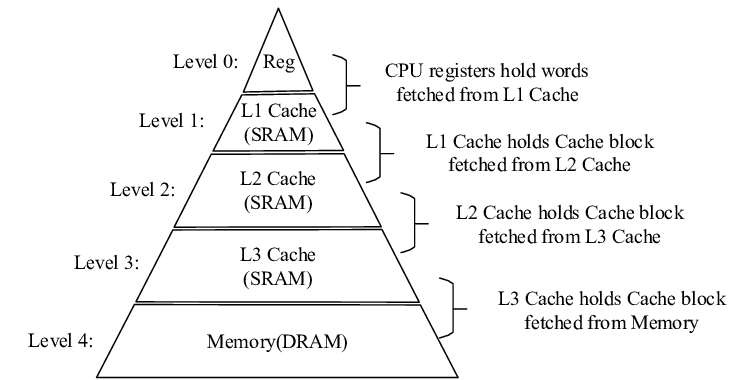
\includegraphics[width=0.90\textwidth]{img/Cache-Hierarchie.png}
    \caption{Klassische Drei-Level Cache Hierarchie}
	\cite{gao_cspm_2022}
    \label{fig:cache_hierarchie}
\end{figure}

\sh{Von Single-Core zum Multi-Core(2000er)}
Mit der Jahrtausendwende stießen Single-Core-Architekturen an physikalische Grenzen: Höhere Taktfrequenzen führten zu überproportionalem Energieverbrauch und Wärmeentwicklung\footnote{Basierend auf dem \textit{Moore’s Law} (Verdopplung der Transistoranzahl auf gleicher Fläche etwa alle zwei Jahre) beschreibt \textit{Dennard Scaling}, dass mit der Verkleinerung von Transistoren sowohl die Taktfrequenz als auch die Transistoranzahl gesteigert werden können, während die Leistung konstant bleibt. Mit weiter fortschreitender Miniaturisierung konnte die Versorgungsspannung jedoch nicht mehr proportional reduziert werden, wodurch Leckströme zunahmen und das Gesetz schließlich zusammenbrach.}. Dies markierte das Ende der \enquote{freien} Leistungssteigerungen durch höhere Frequenzen. Die Antwort der Industrie war die Orientierung zu Parallelismus: Mehrkernprozessoren, \textit{\ac{SMT}} und spezialisierte Hardwareeinheiten ermöglichten weiterhin Leistungszuwächse, allerdings unter deutlich komplexeren Bedingungen für die Softwareentwicklung \parencites[S.~3f]{shalf_new_2007}[S.~67f]{parkhurst_single_2006}.

Parallel dazu nahm die Bedeutung mobiler Endgeräte wie Smartphones und Tablets zu. Mikroprozessoren bildeten hier die Basis, während Fortschritte in der Halbleiterfertigung die hohe Transistordichte und Energieeffizienz dieser Geräte ermöglichten \parencite[S.~2]{hennessy_computer_2011}.

\sh{Rechenzentren, Cloud und neue Software-Paradigmen (2010er)}
Die 2010er Jahre waren geprägt von der Ausbreitung großskaliger Rechenzentren und \textit{Warehouse-Scale Computers}. Diese Systeme setzen nicht mehr auf einzelne Hochleistungsprozessoren, sondern auf die Verwaltung tausender standardisierter Mikroprozessoren in Clustern ausgelegt \parencites[S.~6]{hennessy_computer_2011}[S.~158]{kanev_profiling_2015}[S.~29]{mars_heterogeneity_2011}.

Gleichzeitig veränderte sich die Softwarelandschaft: Produktivität rückte stärker in den Vordergrund, wodurch Sprachen wie Java oder Python populärer wurden, auch wenn dies auf Kosten der maximalen Performance ging \parencite[S.~2]{hennessy_computer_2011}. Mit dem Aufkommen von \textit{\ac{SaaS}} verschoben sich zentrale Rechenprozesse in die Cloud, was neue Anforderungen an Architektur und Skalierbarkeit stellte \parencites[S.~158]{kanev_profiling_2015}[S.~29]{mars_heterogeneity_2011}.

\sh{Aktuelle Entwicklungen: Heterogenität, GPUs und KI (2020er)}
In der Gegenwart zeichnet sich ab, dass \ac{ILP} weitgehend ausgereizt ist. Stattdessen rücken neue Formen der Parallelisierung in den Vordergrund:

\begin{itemize}
    \item \textit{\ac{DLP}} wird durch Vektorprozessoren und \ac{SIMD}-Instruktionen realisiert.
    \item \textit{\ac{TLP}} bleibt durch Multi-Core- und Many-Core-Architekturen bedeutend.
    \item \textit{\ac{DSA}} wie GPUs oder \ac{TPU}s sind auf spezifische Anwendungsfelder optimiert – insbesondere auf das Training und die Inferenz von künstlichen neuronalen Netzen.
\end{itemize}

GPUs, ursprünglich für Grafikberechnungen konzipiert, haben sich als hocheffiziente Plattformen für massiv parallele Berechnungen etabliert und bilden heute das Rückgrat des \textit{Deep Learning}. Spezialisierte KI-Beschleuniger, etwa von Google, NVIDIA oder Apple, treiben die Entwicklung weiter voran. Parallel dazu experimentiert die Forschung mit neuromorphen Architekturen und Quantencomputern, die langfristig völlig neue Paradigmen versprechen.
